\appendixtitleon

\chapter{Artery}

\section{code verification}
\label{app:VV-artery}


In this work, code verification is performed by considering a cube $B = [0,1]^3$ and a manufactured displacement field taken as 
\begin{equation}
    \bfu^{\textnormal{MMS}}(\bfx) = (-0.01\exp(x_3), 0, 0)^T\,.
\end{equation}
Dirichlet boundary conditions in accordance with the above solution are prescribed on all boundaries. A body force is defined such that the manufactured solution corresponds to the nonlinear boundary value problem defined in Section \ref{subsec:def-NBVP}. The convergence order is measured by the $L^2$-norm of the difference between the approximation and the manufactured solution. The $h$-convergence of the norm is shown in Fig.~\ref{fig:mms}, and a third-order convergence rate is observed as expected.
\begin{figure}[ht!]
    \begin{center}
        \includegraphics[trim = {2cm 9cm 2cm 9cm}, clip, width = 0.6\textwidth]{Pictures/MMS-Convergence.pdf}
    \end{center}
    \caption[Convergence of the $L^2$ error for the manufactured solution.]{Convergence of the $L^2$ error ($h$-refinement) for the manufactured solution.}
    \label{fig:mms}
\end{figure}

\section{Strategy for Solving the Fractional Stochastic Partial Differential Equation}\label{sec:solver-SPDE}
For the sake of self-consistency, the numerical strategy to solve the anisotropic fractional stochastic partial differential equation
\begin{equation}
    (\gamma^2 \mathcal{I} -\langle \nabla, \bs{D}\nabla\rangle)^{\alpha/2} U = \dot{W}\,,
    \label{eq:spdeH-app}
\end{equation}
is recalled in this appendix. Following \cite{Lindgren2011}, a finite-dimensional representation associated with a set $\{\psi_i\}_{i=1}^{N}$ of piecewise linear basis functions (with a mesh comprising $N$ nodes) is introduced as follows:
\begin{equation}
U(\bs{x}) = \sum_{i=1}^{N} U_i \psi_i(\bs{x})\,.
\end{equation}
Let $\bs{U} = (U_1, \ldots, U_N)^T$ be the Gaussian random vector of nodal values. For $\alpha = 2$, it was shown in the above reference that the weak Galerkin stochastic solution satisfies
\begin{equation}
    \bs{U} \sim \mathcal{N}(\bs{0}_N, \bs{\Sigma})\,,
\end{equation}
where the covariance matrix $\bs{\Sigma}$ is given by 
\begin{equation}
    \bs{\Sigma} = \left(\kappa^2 \bs{M} + \bs{G}\right)^{-1} \bs{M} \left(\kappa^2 \bs{M} + \bs{G}\right)^{-1}]\,,
\end{equation} 
with
\begin{equation}
M_{ij} = \int_{\Omega} \psi_i(\bs{x})\psi_j(\bs{x})\,d\bs{x}
\label{eq:M}
\end{equation}
and
\begin{equation}
G_{ij} = \int_{\Omega} \langle \bs{\nabla}\psi_i(\bs{x}), \bs{D}(\bs{x})\bs{\nabla}\psi_j(\bs{x})\rangle \, d\bs{x}
\end{equation}
for $1 \leqslant i,j \leqslant N$, respectively. For computational efficiency, the sampling task is then usually recast using the precision matrix 
\begin{equation}
    \bs{\Sigma}^{-1} = \left(\kappa^2 \bs{M} + \bs{G}\right) \bs{M}^{-1} \left(\kappa^2 \bs{M} + \bs{G}\right)\,,
\end{equation}
where $\bs{M}^{-1}$ can be evaluated by applying a lumping procedure. For $\alpha \neq 2$, recursive formula can be applied, see \cite{Lindgren2011}.

\chapter{Nonlinear-Manifold Reduced-Order Model and Operator Learning}
\section{Reduced-Order Model Solutions}
In this Appendix, additional solution snapshots are provided, together with absolute errors, to assess the accuracy of the presented frameworks.
\begin{figure}[!htb]
     \begin{center}
        \begin{subfigure}[b]{0.23\textwidth}
            \begin{center}
                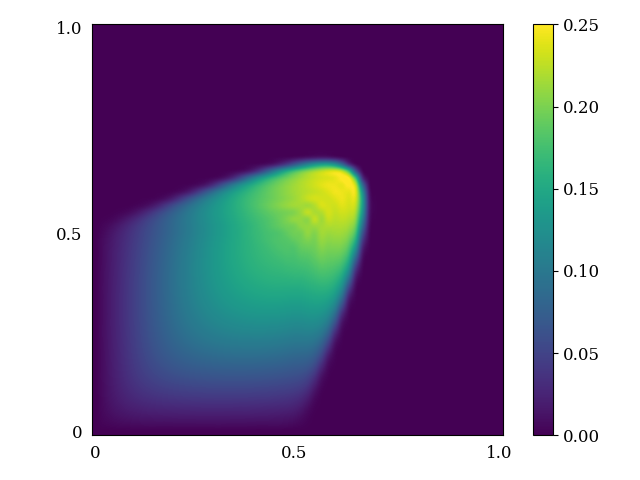
\includegraphics[trim = {0, 0, 3cm, 0}, clip, width=\textwidth]{Pictures/X-rom-LE-DAE-5.png}
            \end{center}
            \caption{Solution $r = 5$}
        \end{subfigure}
   \begin{subfigure}[b]{0.23\textwidth}
            \begin{center}
                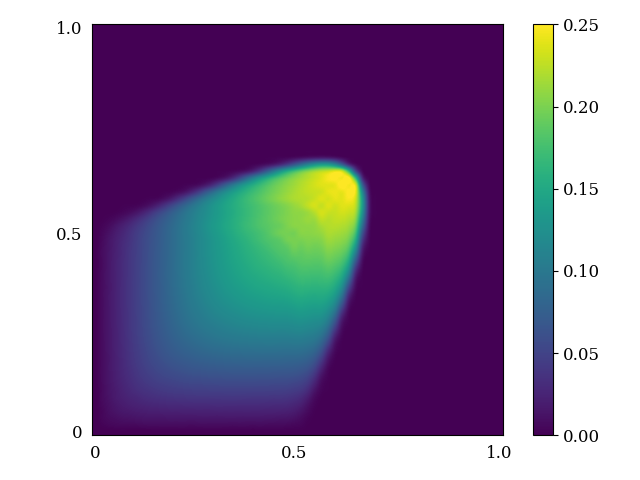
\includegraphics[trim = {0, 0, 3cm, 0}, clip, width=\textwidth]{Pictures/X-rom-LE-DAE-10.png}
            \end{center}
            \caption{Solution $r = 10$}
        \end{subfigure}
   \begin{subfigure}[b]{0.23\textwidth}
            \begin{center}
                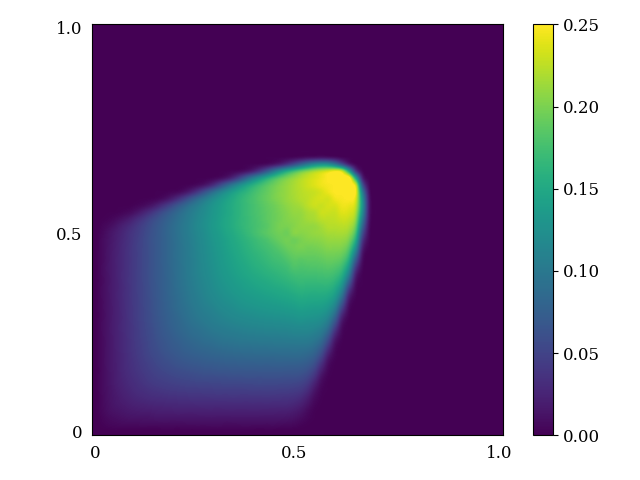
\includegraphics[trim = {0, 0, 3cm, 0}, clip, width=\textwidth]{Pictures/X-rom-LE-DAE-15.png}
            \end{center}
            \caption{Solution $r = 15$}
        \end{subfigure}
   \begin{subfigure}[b]{0.23\textwidth}
            \begin{center}
                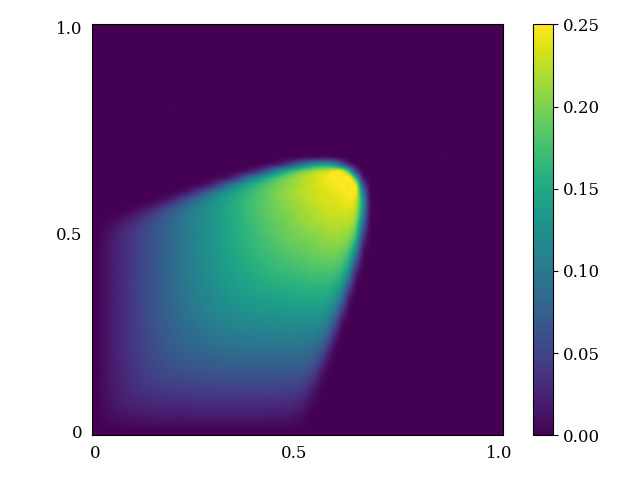
\includegraphics[trim = {0, 0, 3cm, 0}, clip, width=\textwidth]{Pictures/X-rom-LE-DAE-20.png}
            \end{center}
            \caption{Solution $r = 20$}
        \end{subfigure}\\  
        \begin{subfigure}[b]{0.23\textwidth}
            \begin{center}
                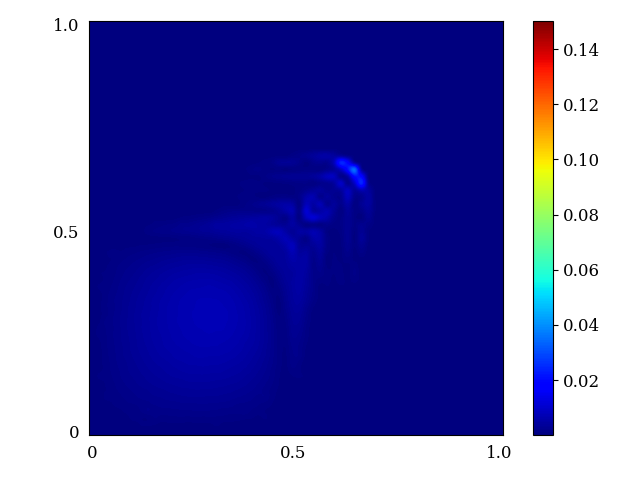
\includegraphics[trim = {0, 0, 3cm, 0}, clip, width=\textwidth]{Pictures/X-rom-LE-DAE-5-abs-err.png}
            \end{center}
            \caption{Absolute error $r = 5$}
        \end{subfigure}  
        \begin{subfigure}[b]{0.23\textwidth}
            \begin{center}
                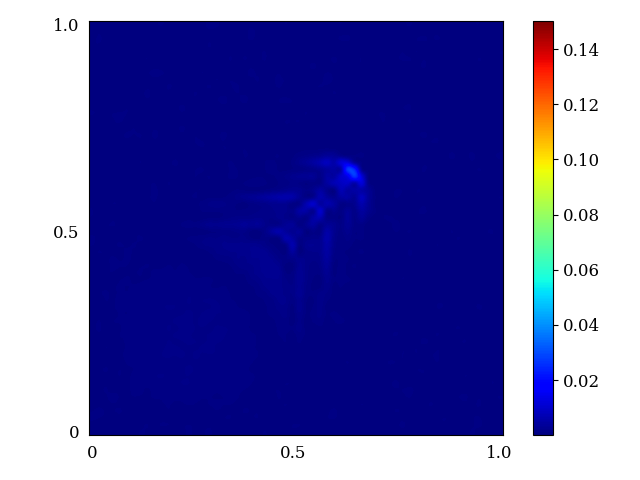
\includegraphics[trim = {0, 0, 3cm, 0}, clip, width=\textwidth]{Pictures/X-rom-LE-DAE-10-abs-err.png}
            \end{center}
            \caption{Absolute error $r = 10$}
        \end{subfigure}   
        \begin{subfigure}[b]{0.23\textwidth}
            \begin{center}
                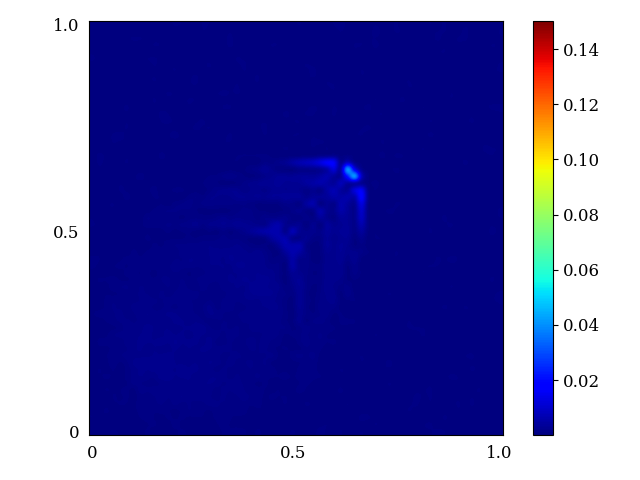
\includegraphics[trim = {0, 0, 3cm, 0}, clip, width=\textwidth]{Pictures/X-rom-LE-DAE-15-abs-err.png}
            \end{center}
            \caption{Absolute error $r = 15$}
        \end{subfigure}    
        \begin{subfigure}[b]{0.23\textwidth}
            \begin{center}
                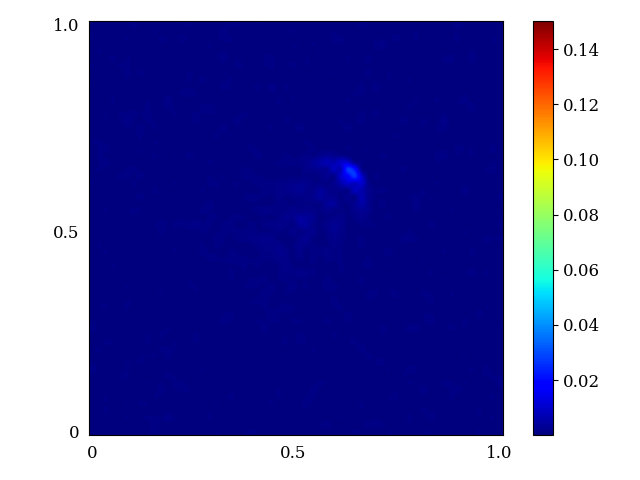
\includegraphics[trim = {0, 0, 3cm, 0}, clip, width=\textwidth]{Pictures/X-rom-LE-DAE-20-abs-err.png}
            \end{center}
            \caption{Absolute error $r = 20$}
        \end{subfigure}
     \end{center}
     \caption[Solutions and pointwise errors for LE-DAE-DNNOp.]{Solutions (a, b, c, d) and pointwise errors (e, f, g, h) for LE-DAE-DNNOp with different latent space dimensions.}
        \label{fig: ledae-burger}
\end{figure}

\begin{figure}[!htb]
     \begin{center}
        \begin{subfigure}[b]{0.23\textwidth}
            \begin{center}
                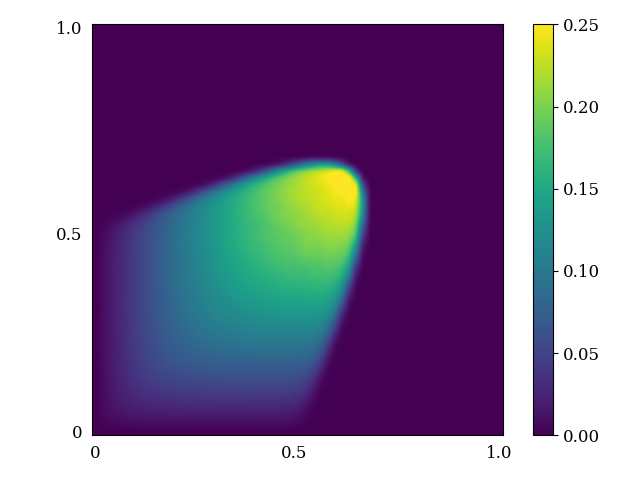
\includegraphics[trim = {0, 0, 3cm, 0}, clip, width=\textwidth]{Pictures/X-rom-LE-SAE-5.png}
            \end{center}
            \caption{Solution $r = 5$}
        \end{subfigure}
   \begin{subfigure}[b]{0.23\textwidth}
        \begin{center}
            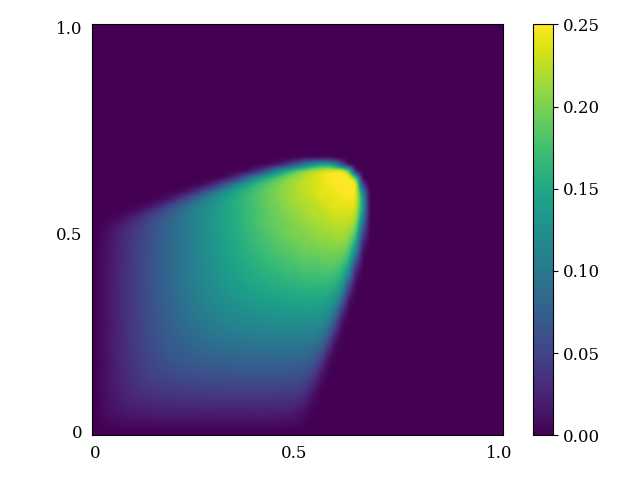
\includegraphics[trim = {0, 0, 3cm, 0}, clip, width=\textwidth]{Pictures/X-rom-LE-SAE-10.png}
        \end{center}
            \caption{Solution $r = 10$}
        \end{subfigure}
   \begin{subfigure}[b]{0.23\textwidth}
       \begin{center}
        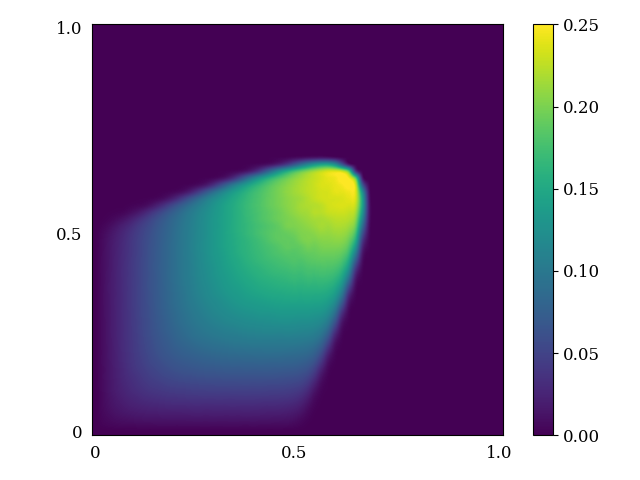
\includegraphics[trim = {0, 0, 3cm, 0}, clip, width=\textwidth]{Pictures/X-rom-LE-SAE-15.png}
       \end{center}
            \caption{Solution $r = 15$}
        \end{subfigure}
   \begin{subfigure}[b]{0.23\textwidth}
       \begin{center}
        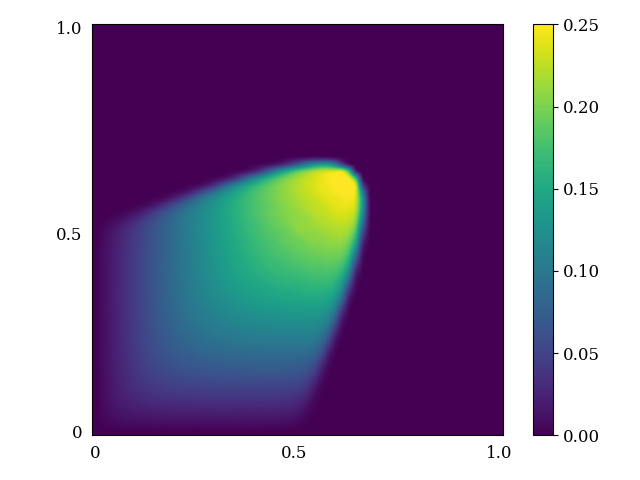
\includegraphics[trim = {0, 0, 3cm, 0}, clip, width=\textwidth]{Pictures/X-rom-LE-SAE-20.png}
       \end{center}
            \caption{Solution $r = 20$}
        \end{subfigure}\\  
        \begin{subfigure}[b]{0.23\textwidth}
            \begin{center}
                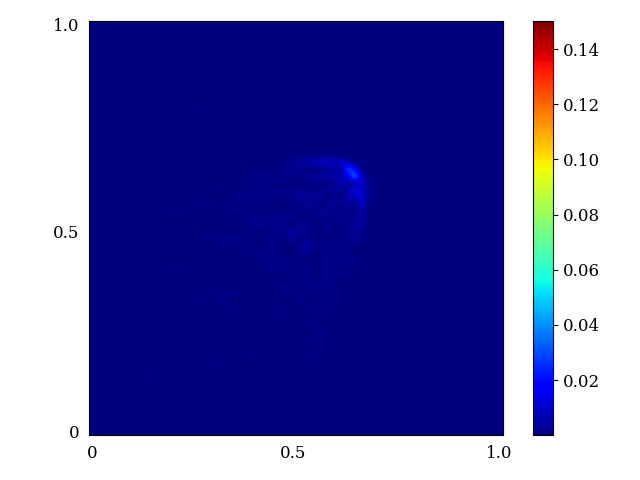
\includegraphics[trim = {0, 0, 3cm, 0}, clip, width=\textwidth]{Pictures/X-rom-LE-SAE-5-abs-err.png}
            \end{center}
            \caption{Absolute error $r = 5$}
        \end{subfigure}  
        \begin{subfigure}[b]{0.23\textwidth}
            \begin{center}
                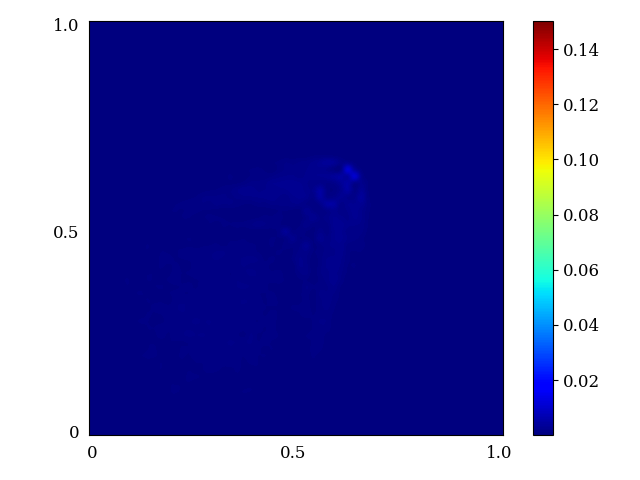
\includegraphics[trim = {0, 0, 3cm, 0}, clip, width=\textwidth]{Pictures/X-rom-LE-SAE-10-abs-err.png}
            \end{center}
            \caption{Absolute error $r = 10$}
        \end{subfigure}   
        \begin{subfigure}[b]{0.23\textwidth}
            \begin{center}
                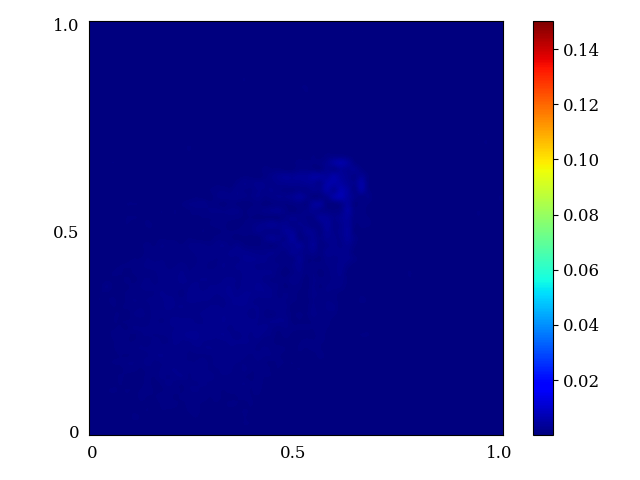
\includegraphics[trim = {0, 0, 3cm, 0}, clip, width=\textwidth]{Pictures/X-rom-LE-SAE-15-abs-err.png}
            \end{center}
            \caption{Absolute error $r = 15$}
        \end{subfigure}    
        \begin{subfigure}[b]{0.23\textwidth}
            \begin{center}
                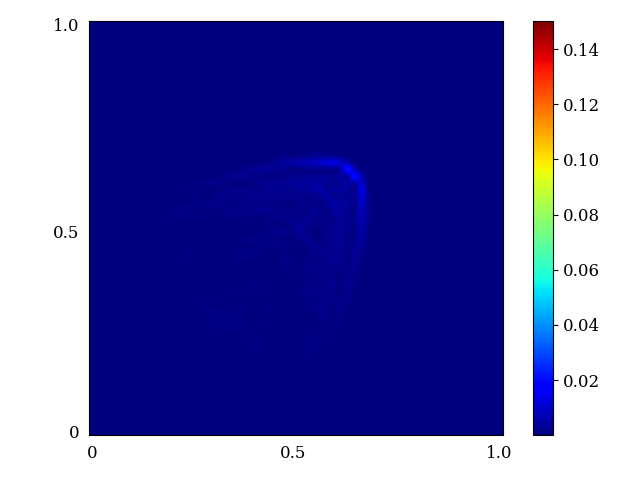
\includegraphics[trim = {0, 0, 3cm, 0}, clip, width=\textwidth]{Pictures/X-rom-LE-SAE-20-abs-err.png}
            \end{center}
            \caption{Absolute error $r = 20$}
        \end{subfigure}
     \end{center}
     \caption[Solutions and pointwise errors for LE-SAE-DNNOp.]{Solutions (a, b, c, d) and pointwise errors (e, f, g, h) for LE-SAE-DNNOp with different latent space dimensions.}
        \label{fig: lesae-burger}
\end{figure}


\begin{figure}[!htb]
     \begin{center}
        \begin{subfigure}[b]{0.23\textwidth}
            \begin{center}
                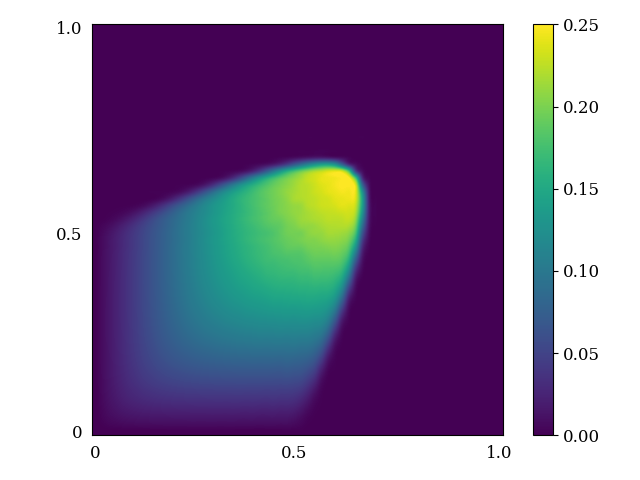
\includegraphics[trim = {0, 0, 3cm, 0}, clip, width=\textwidth]{Pictures/X-rom-LE-CNNAE-5.png}
            \end{center}
             \caption{Solution $r = 5$}
         \end{subfigure}
    \begin{subfigure}[b]{0.23\textwidth}
            \begin{center}
                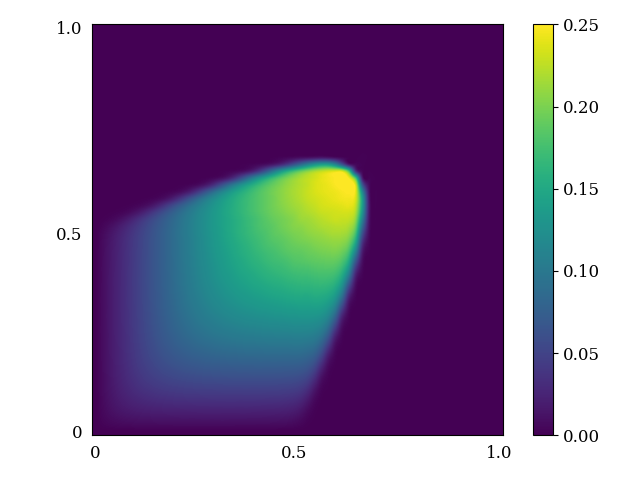
\includegraphics[trim = {0, 0, 3cm, 0}, clip, width=\textwidth]{Pictures/X-rom-LE-CNNAE-10.png}
            \end{center}
             \caption{Solution $r = 10$}
         \end{subfigure}
    \begin{subfigure}[b]{0.23\textwidth}
            \begin{center}
                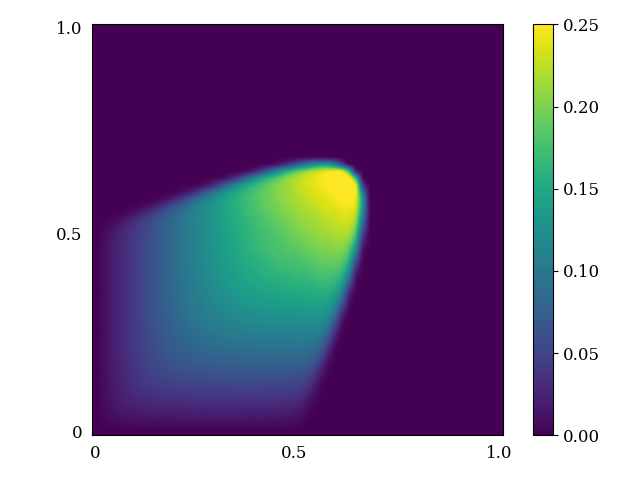
\includegraphics[trim = {0, 0, 3cm, 0}, clip, width=\textwidth]{Pictures/X-rom-LE-CNNAE-15.png}
            \end{center}
             \caption{Solution $r = 15$}
         \end{subfigure}
    \begin{subfigure}[b]{0.23\textwidth}
            \begin{center}
                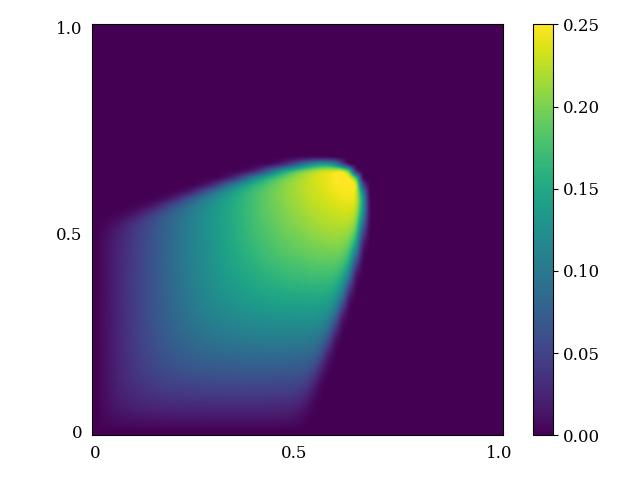
\includegraphics[trim = {0, 0, 3cm, 0}, clip, width=\textwidth]{Pictures/X-rom-LE-CNNAE-20.png}
            \end{center}
             \caption{Solution $r = 20$}
         \end{subfigure}\\  
         \begin{subfigure}[b]{0.23\textwidth}
             \begin{center}
                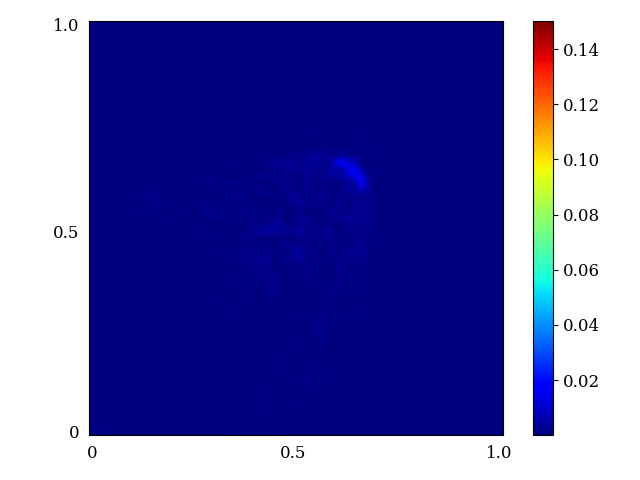
\includegraphics[trim = {0, 0, 3cm, 0}, clip, width=\textwidth]{Pictures/X-rom-LE-CNNAE-5-abs-err.png}
             \end{center}
             \caption{Absolute error $r = 5$}
         \end{subfigure}  
         \begin{subfigure}[b]{0.23\textwidth}
             \begin{center}
                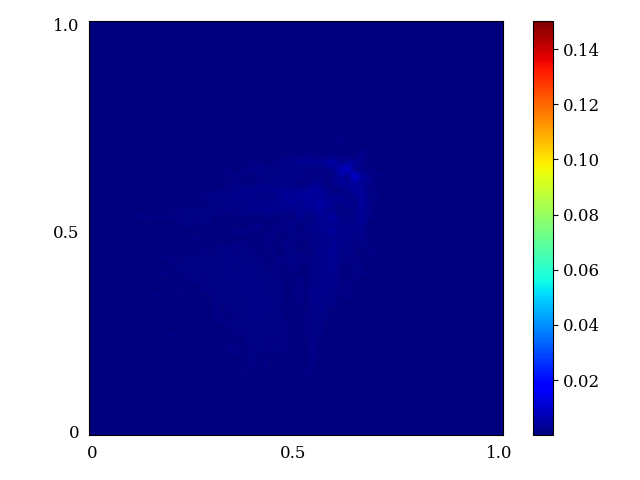
\includegraphics[trim = {0, 0, 3cm, 0}, clip, width=\textwidth]{Pictures/X-rom-LE-CNNAE-10-abs-err.png}
             \end{center}
             \caption{Absolute error $r = 10$}
         \end{subfigure}   
         \begin{subfigure}[b]{0.23\textwidth}
             \begin{center}
                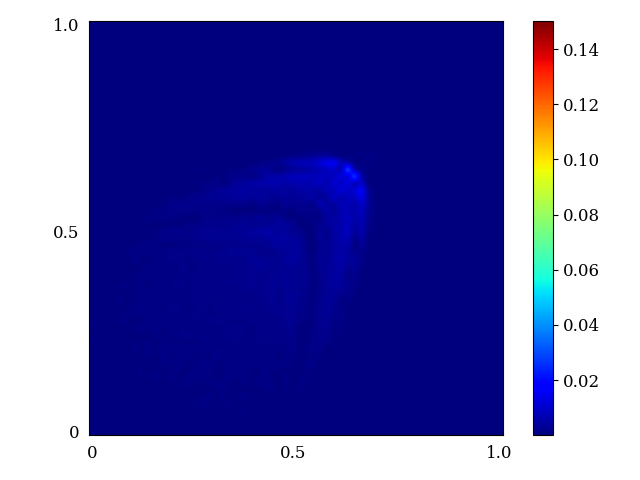
\includegraphics[trim = {0, 0, 3cm, 0}, clip, width=\textwidth]{Pictures/X-rom-LE-CNNAE-15-abs-err.png}
             \end{center}
             \caption{Absolute error $r = 15$}
         \end{subfigure}    
         \begin{subfigure}[b]{0.23\textwidth}
             \begin{center}
                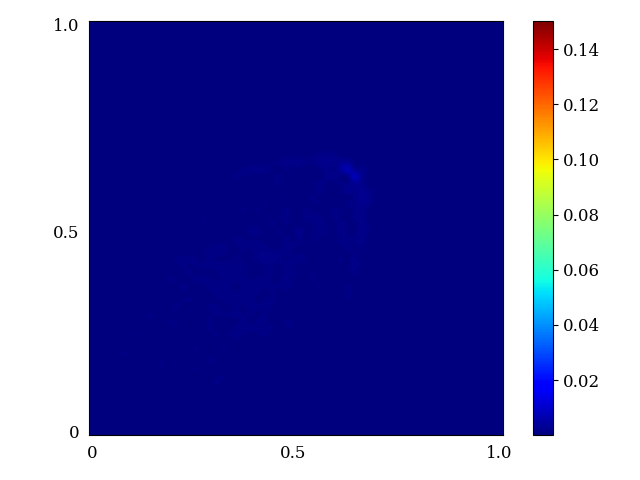
\includegraphics[trim = {0, 0, 3cm, 0}, clip, width=\textwidth]{Pictures/X-rom-LE-CNNAE-20-abs-err.png}
             \end{center}
             \caption{Absolute error $r = 20$}
         \end{subfigure}
     \end{center}
     \caption[Solutions and pointwise errors for LE-CNNAE-DNNOp.]{Solutions (a, b, c, d) and pointwise errors (e, f, g, h) for LE-CNNAE-DNNOp with different latent space dimensions.}
        \label{fig: lecnnae-burger}
\end{figure}

\begin{figure}[!htb]
     \begin{center}
        \begin{subfigure}[b]{0.23\textwidth}
       \begin{center}
        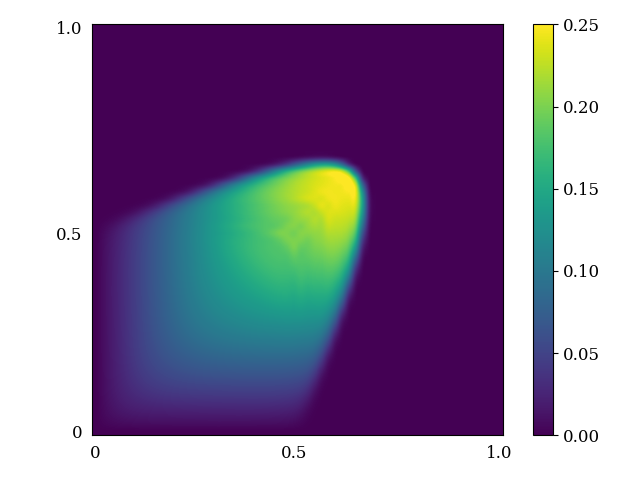
\includegraphics[trim = {0, 0, 3cm, 0}, clip, width=\textwidth]{Pictures/X-rom-NE-DAE-5.png}
       \end{center}
            \caption{Solution $r = 5$}
        \end{subfigure}
   \begin{subfigure}[b]{0.23\textwidth}
        \begin{center}
            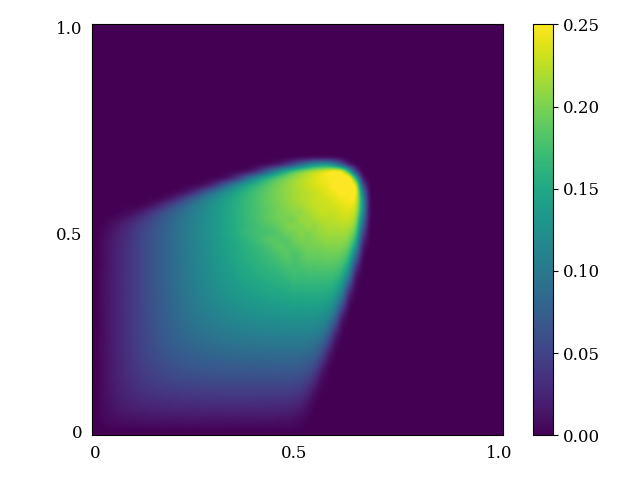
\includegraphics[trim = {0, 0, 3cm, 0}, clip, width=\textwidth]{Pictures/X-rom-NE-DAE-10.png}
        \end{center}
            \caption{Solution $r = 10$}
        \end{subfigure}
   \begin{subfigure}[b]{0.23\textwidth}
            \begin{center}
                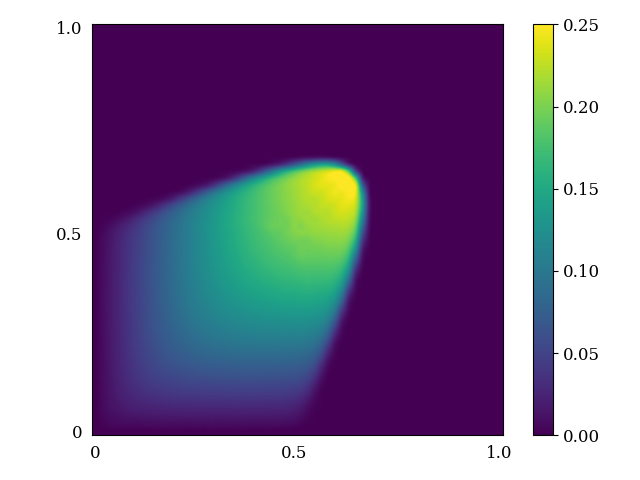
\includegraphics[trim = {0, 0, 3cm, 0}, clip, width=\textwidth]{Pictures/X-rom-NE-DAE-15.png}
            \end{center}
            \caption{Solution $r = 15$}
        \end{subfigure}
   \begin{subfigure}[b]{0.23\textwidth}
            \begin{center}
                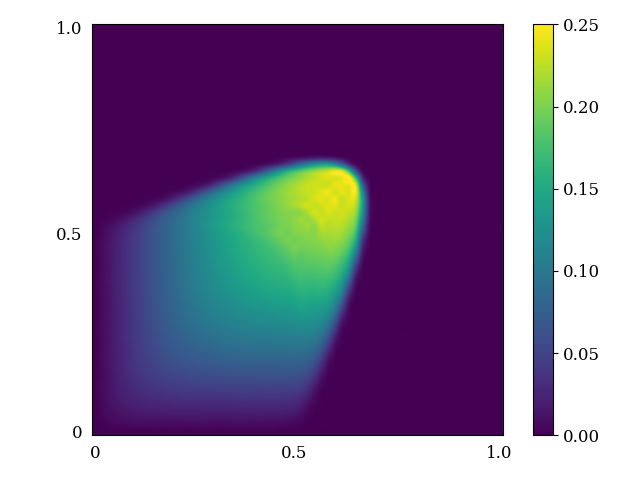
\includegraphics[trim = {0, 0, 3cm, 0}, clip, width=\textwidth]{Pictures/X-rom-NE-DAE-20.png}
            \end{center}
            \caption{Solution $r = 20$}
        \end{subfigure}\\  
        \begin{subfigure}[b]{0.23\textwidth}
            \begin{center}
                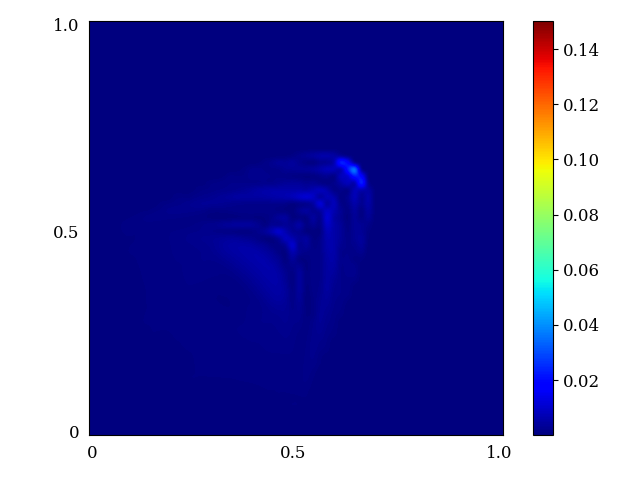
\includegraphics[trim = {0, 0, 3cm, 0}, clip, width=\textwidth]{Pictures/X-rom-NE-DAE-5-abs-err.png}
            \end{center}
            \caption{Absolute error $r = 5$}
        \end{subfigure}  
        \begin{subfigure}[b]{0.23\textwidth}
            \begin{center}
                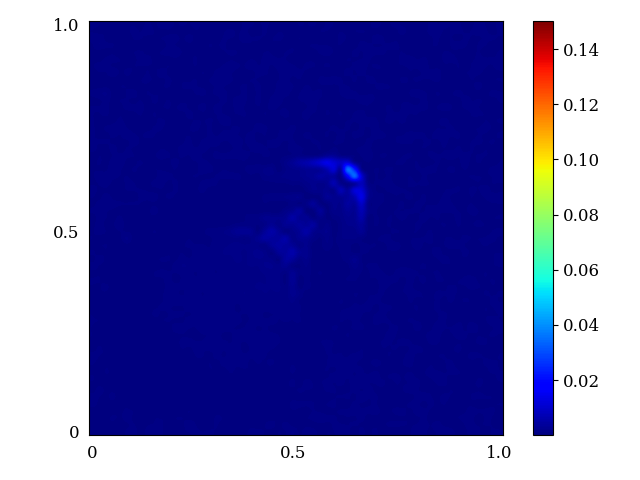
\includegraphics[trim = {0, 0, 3cm, 0}, clip, width=\textwidth]{Pictures/X-rom-NE-DAE-10-abs-err.png}
            \end{center}
            \caption{Absolute error $r = 10$}
        \end{subfigure}   
        \begin{subfigure}[b]{0.23\textwidth}
            \begin{center}
            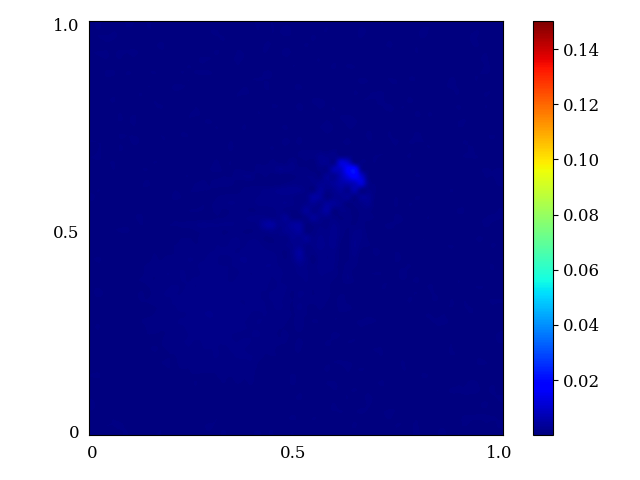
\includegraphics[trim = {0, 0, 3cm, 0}, clip, width=\textwidth]{Pictures/X-rom-NE-DAE-15-abs-err.png}
            \end{center}
            \caption{Absolute error $r = 15$}
        \end{subfigure}    
        \begin{subfigure}[b]{0.23\textwidth}
            \begin{center}
                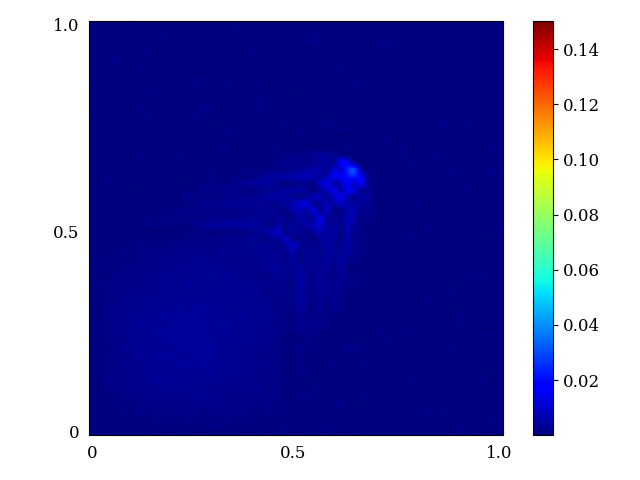
\includegraphics[trim = {0, 0, 3cm, 0}, clip, width=\textwidth]{Pictures/X-rom-NE-DAE-20-abs-err.png}
            \end{center}
            \caption{Absolute error $r = 20$}
        \end{subfigure}
     \end{center}
     \caption[Solutions and pointwise errors for NE-DAE-DNNOp.]{Solutions (a, b, c, d) and pointwise errors (e, f, g, h) for NE-DAE-DNNOp with different latent space dimensions.}
        \label{fig: nedae-burger}
\end{figure}

\chapter{Concurrent Multiscale Simulations of Nonlinear Random Materials Using Probabilistic Learning}

\section{Formulas for Conditional Statistics}
\label{app:fe2}

In this Appendix, we use the following notation. The real-valued random variable $Q$ denotes any component of the $\RR^{n_q}$-valued random variable $\bfQ$, and the real variable $q$ represents the corresponding component of the vector $\bfq$ in $\RR^{n_q}$.
%
Let $\widetilde{Q}$ and $\widetilde{\bfW} = (\widetilde{W}_{1},\ldots,\widetilde{W}_{n_w})$ be the normalized random variables defined by
%
\begin{equation}\label{eqPLoMA1}
    \widetilde{Q} = (Q - \underline{q}) /{{\sigma_{\! Q}}}\quad , \quad
    \widetilde{W}_k = (W_k - \underline{w}_k) /{{\sigma_{W_k}}} \quad , \quad k=1,\ldots, n_w \,,
\end{equation}
%
where $\underline{q}$, $\underline{w}_k$, and $\sigma_{\! Q}$, $\sigma_{W_k}$ are the mean values and standard deviations of the random variables $Q$ and $W_k$. These values are estimated using empirical statistical estimators based on the learned realizations $\{(\bfq_\ar^\ell,\bfw_\ar^\ell), \ell = 1,\ldots,n_\ar\}$.
%
For any value $\bfw_0 = (w_{0,1},\ldots , w_{0,n_w})$ of the control parameter given in $\curC_w\subset\RR^{n_w}$, we define the vector $\widetilde\bfw_0$ in $\RR^{n_w}$ such that
%
\begin{equation}\label{eqPLoMA2}
 \widetilde{w}_{0,k} = (w_{0,k} - \underline{w}_k) /{\sigma_{W_k}} \quad , \quad k=1,\ldots, n_w \,.
\end{equation}
%
The Gaussian KDE estimation of the joint probability distribution of $\widetilde Q$ and $\widetilde{\bfW}$, with respect to 
$d\widetilde{q}\, d\widetilde{\bfw}$, is written as 
%
\begin{equation}\label{eqPLoMA3}
    \textit{p}_{\widetilde{Q},\widetilde{\bfW}}(\widetilde{q},\widetilde{\bfw}) 
    = \frac{1}{n_\ar}\sum_{\ell = 1}^{n_\ar} \frac{1}{\sqrt{2\pi} s} \exp({-\frac{1}{2s^2}( \widetilde{q} - \widetilde{q}^\ell_\ar )^2})
     \frac{1}{(\sqrt{2\pi}s)^{\pppcarac{n_w}}}
     \exp({-\frac{1}{2s^2}\Vert \widetilde{\bfw} - \widetilde{\bfw}^\ell_\ar \Vert^2})\, .
\end{equation}
%
In Eq.~\eqref{eqPLoMA3}, $s$ is the Silverman bandwidth defined by 
%
\begin{equation}\label{eqPLoMA4}
    s = \left\{\frac{4}{n_\ar(2+n)} \right\}^{1/(n + 4)}\quad ,\quad n = 1 + n_w \,,
\end{equation}
%
and, for $\ell=1,\ldots , n_\ar$, $\widetilde{q}_\ar^\ell$ and $\widetilde{w}^\ell_{\ar,k}$ are defined by
%
\begin{equation}\label{eqPLoMA5}
    \widetilde{q}_\ar^\ell = (q_\ar^\ell - \underline{q}) /{{\sigma_{\! Q}}}\quad , \quad
    \widetilde{w}^\ell_{\ar,k} = ({w}^\ell_{\ar,k} - \underline{w}_k) /{{\sigma_{W_k}}} \quad , \quad k=1,\ldots, n_w \,.
\end{equation}
%
From Eq.~\eqref{eqPLoMA3}, the following formulas for conditional statistics are derived.\\

\noindent {\it (i)} The conditional mathematical expectation $E\{Q \, \vert \, \bfW = \bfw_o\}$ of $Q$ given $\bfW = \bfw_0$ in $\curC_w$ is given by
%
\begin{equation}
    E\{Q \, \vert \, \bfW = \bfw_0\} = \underline{q} + \sigma_{\! Q}\, \frac{\sum_{\ell=1}^{n_\ar}\widetilde{q}^{\ell}_{\ar} \times \exp({-\frac{1}{2s^2}\Vert \widetilde{\bfw}_{0}  -\widetilde{\bfw}^\ell_\ar \Vert^2})}{\sum_{\ell =  1}^{n_\ar}\exp({-\frac{1}{2s^2}\Vert \widetilde{\bfw}_{0} - \widetilde{\bfw}^\ell_\ar \Vert^2})} \,.
     \label{eqPLoM6}
\end{equation}
%

\noindent {\it (ii)} The conditional probability density function  $p_{Q \vert \bfW} (q\, \vert \, \bfw_0)$ with respect to $dq$ of $Q$ given $\bfW = \bfw_0$ in $\curC_w$ is defined as
%
\begin{equation}
      p_{Q \vert \bfW} (q\, \vert \, \bfw_0)  = \frac{1}{\sqrt{2\pi}\,  s \,\sigma_{\! Q}}
      \frac{\sum_{\ell=1}^{n_\ar}
       \exp({-\frac{1}{2s^2}( \widetilde{q} - \widetilde{q}^\ell_\ar )^2})      
      \times \exp({-\frac{1}{2s^2}\Vert \widetilde{\bfw}_{0}  -\widetilde{\bfw}^\ell_\ar \Vert^2})}{\sum_{\ell =  1}^{n_\ar}\exp({-\frac{1}{2s^2}\Vert \widetilde{\bfw}_{0} - \widetilde{\bfw}^\ell_\ar \Vert^2})} \quad , \quad
      \widetilde{q} = (q - \underline{q}) /{{\sigma_{\! Q}}} \, .
     \label{eqPLoM7}
\end{equation}
%

\noindent {\it (iii)} The conditional cumulative distribution function $F_{Q \vert \bfW}(q^*\vert\bfw_{0}) 
= \rm{Proba}\{Q\leq q^*\,\vert\,\bfW = \bfw_0 \}$ of $Q$ given $\bfW = \bfw_0$ in $\curC_w$ is estimated using
%
\begin{equation}\label{eqPLoMA8}
    F_{Q\vert\bfW}(q^* \vert \bfw_0 ) 
    = \frac{ \sum_{\ell=1}^{n_\ar} \widetilde{F}^\ell (\widetilde{q}^*) \times 
              \exp( -\frac{1}{2s^2} \Vert \widetilde{\bfw}_{0} - \widetilde{\bfw}^\ell \Vert^2 ) }
           { \sum_{\ell = 1}^{n_\ar} \exp( -\frac{1}{2s^2} \Vert \widetilde{\bfw}_{0} - \widetilde{\bfw}^\ell \Vert^2) } \quad , \quad \widetilde{q}^* = (q^* - \underline{q}) / \sigma_{\! Q}\,,
\end{equation}
with
\begin{equation}\label{eqPLoMA9}
    \widetilde{F}^\ell (\widetilde{q}^*) = \frac{1}{2} + \frac{1}{2}
    \erf(\frac{1}{\sqrt{2}\,s} ( \widetilde{q}^* - \widetilde{q}^\ell_{\ar} ) )
    \quad , \quad \erf(y) = \frac{2}{\sqrt{\pi}}\int_{0}^{y} e^{-t^2}\, dt \, .
\end{equation}